\section{Overview}
The northport kernel is a modular-monolithic design. The kernel itself is a single binary providing most of the functionally required for the system to run, while drivers are loaded as dynamically linked modules. The kernel is written mostly in C++, with some platform-specific assembly where appropriate.

\subsection{Subsystems and Layers}
The kernel consists of a series of major and supporting subsystems, organised into various layers. The source code is generally organised by subsystem, and the distinction between layers is mainly visible in how the code interacts with other code.

Layers exist as a distinction in kernel logic: code in one layer can be aware of other code in the same layer and lower layers, but not code in higher layers. As with any rule there are some special cases where an exception is made, but special care is taken in these and no assumptions are made about the state of the higher-layer code. Layers can also be thought of a representation of complexity, with lower layers providing more basic functionality and higher layers providing more abstract things.

\paragraph{Major Subsystems}
\begin{itemize}
    \item Memory management stack: Contains the physical memory manager, virtual memory manager and it's virtual memory drivers, as well as providing the general purpose heap.
    \item Interrupt infrastructure: Interrupt vector allocation, interrupt dispatch, and handling the effects of changing the core run level (switching to DPCs, etc).
    \item Timekeeping: The system clock lives here and provides functions for up-counting software timers (\textit{stopwatches}) and enqueuing callback functions to run after a specified time (\textit{clock events}).
    \item Program management and Scheduling: this contains the scheduler, as well as threads and processes, and ways to manage them.
    \item Hardware detection: includes the device tree parser and code for parsing ACPI tables. Support for an AML interpreter (as a loadable driver) is planned in the future.
    \item Devices and Drivers: provides high level functions for managing and communicating with driver programs. The device API is also defined here.
    \item Filesystem and File Cache: contains the VFS, a tempFS implementation (in-memory filesystem with no backing media) and a page-cache system referred to as the \textit{file cache}.
    \item Debugging: TODO:
\end{itemize}

\paragraph{Kernel Layers}
\begin{itemize}
    \item Arch: this layer is tied very closely to the target hardware the kernel is running on. It acts as the glue between the hardware and the functions defined the headers at \verb|include/arch/|, which the rest of the kernel is built upon. The arch layer is comparable to the \textit{HAL} (hardware abstraction layer) that some other systems use.
    \item Core: the core layer contains low level code like the arch layer, but everything here is platform-agnostic. Things like the PMM and VMM live here as most other kernel subsystems are built on top of them. Some parts of the interrupt infrastructure also live here, as does the scheduler.
    \item Support: The support layer provides high level functions like IPC, the VFS and tempFS, program management and driver management.
    \item Drivers: This layer represents privileged programs running as drivers managed by the kernel. The code in this layer is highly dependent on the detected hardware and how the system is configured by it's user.
    \item User: not technically a layer of the kernel, but it is a useful concept. This layer represents any programs running under supervision from the kernel: userspace programs.
\end{itemize}

\begin{figure}[h]
\centering
\begin{tikzpicture}
    \node (archlayer) [rectangle, minimum width=14cm, minimum height=2cm, draw=black, fill=blue!10] {Arch Layer};
    \node (corelayer) [rectangle, minimum width=14cm, minimum height=2cm, draw=black, fill=orange!10, above=1mm of archlayer] {Core Layer};
    \node (supportlayer) [rectangle, minimum width=14cm, minimum height=2cm, draw=black, fill=red!10, above=1mm of corelayer] {Support Layer};
\end{tikzpicture}
\caption{Kernel Layers}
\end{figure}
TODO: diagram of kernel layers

\subsection{Kernel Initialization}
The entry point of the kernel is specific to each architecture, as even with the limine protocol there are still critical differences to account for. The entry function is highly specific to the target architecture, and so it's hard to generalize it in documentation - if you're interested in how a system arch is setup, the best resource will be to check the code.

Having said that, the majority of the init logic for the kernel is shared across all platforms, and is split into stages. The current stage isn't tracked anyway, but progressing to the next stage is represented by calling the next \verb|InitXYZ()| function defined in \verb|kernel/include/CommonInit.h|. Each of these functions brings up another collection of kernel components.

The init code was organised this way to give the freedom of implementation to the architecture-specific parts of the code, which is where it feels the most useful. The guiding principle here was to keep the general kernel code clean, while letting the arch-specific code take care of the messy things.

\begin{figure}[h]
\begin{tikzpicture}
    \node (ApEntry) [rectangle, minimum height=1.5cm, draw=black, fill=blue!10] {
        \verb|ApEntry()|};
    \node (KernelEntry) [rectangle, minimum height=1.5cm, draw=black, fill=blue!10, below = of ApEntry] {
        \verb|KernelEntry()|};
    \node (hidden) [left = 2cm of KernelEntry] {};
    \node (InitCore) [rectangle, minimum height=1.5cm, draw=black, fill=blue!10, right = 3mm of ApEntry] {
        \verb|InitCore()|};
    \node (SchedulerExec) [rectangle, minimum height=1.5cm, draw=black, fill=gray!10, right = of InitCore] {
        Scheduled execution
    };
    \node (InitEarlyPlatform) [rectangle, minimum height=1.5cm, draw=black, fill=gray!10, below = of KernelEntry] {
        \verb|InitEarlyPlatform()|};
    \node (InitMemory) [rectangle, minimum height=1.5cm, draw=black, fill=gray!10, right = 3mm of InitEarlyPlatform] {
        \verb|InitMemory()|};
    \node (InitPlatform) [rectangle, minimum height=1.5cm, draw=black, fill=gray!10, right = 3mm of InitMemory] {
    \verb|InitPlatform()|};

    \path [->, red, dashed] (hidden) edge (KernelEntry.west) node [label=above:Bootloader exit]{};
    \path [->] (KernelEntry.south) edge (InitEarlyPlatform);
    \path [->, in=150, out=-30] (KernelEntry.south) edge (InitMemory.north);
    \path [->, in=140, out=-10] (KernelEntry.south) edge (InitPlatform.north);
    \path [->, red, dashed] (KernelEntry) edge (ApEntry);
    \path [->, bend right, blue!80] (KernelEntry) edge (InitCore);
    \path [->, blue!80] (ApEntry) edge (InitCore);
    \path [->] (InitCore) edge (SchedulerExec);
\end{tikzpicture}

\centering
\begin{tabular}{c|c|l}
    \begin{tikzpicture}
        \path [->, red, dashed] (0, 0) edge (1, 0);
    \end{tikzpicture} 
    & 
    & Platform-specific mechanism. \\

    \begin{tikzpicture}
        \path [->, blue!80] (0, 0) edge (1, 0);
    \end{tikzpicture} 
    & 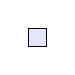
\begin{tikzpicture} \node (r)[rectangle, draw=black, fill=blue!10] (0, 0){}; \end{tikzpicture} 
    & (Call to) platform specific code. \\

    \begin{tikzpicture}
        \path [->, black] (0, 0) edge (1, 0);
    \end{tikzpicture} 
    & 
\begin{tikzpicture} \node (r)[rectangle, draw=black, fill=gray!10] (0, 0){}; \end{tikzpicture}
    & (Call to) common init code. \\
\end{tabular}
\caption{Kernel initialization sequence.}
\end{figure}

\subsection{Multi-Core Operation}
The kernel takes full advantage of multiple processor cores in a system. Most kernel subsystems operate without specific knowledge of how many cores are present in the system, and those that do are only interested in \textit{online} cores. For completeness, a core can also be considered offline (not present or not available to the kernel), or in an initialization state (running kernel code but not ready for general use).

\textit{Currently the kernel brings all cores online when booting, but the kernel is built around the idea that the number of online cores is dynamic - i.e. hotplugging processors at runtime. This feature isn't implemented yet, but provisions have been made.}

As mentioned the bulk of the kernel operates without caring for the number of online cores in the system. This becomes a little blurry when performance of some subsystems becomes involved, where often per-core resource caches are created to reduce contention between cores. The implementation of these caches this breaks the idea of not caring about the number of cores, but the illusion remains from the consuming code's point of view. These per-core caches can also be disabled with feature flags if desired.

If for some reason some code \textbf{must} execute on a particular core, there are two options: the IPI mailboxes or pinning a thread to a particular core. IPI mailboxes are useful for time sensitive actions as writing to a mailbox triggers an interrupt on the receiving core.

\paragraph{Topology Awareness}
If available, the kernel also tracks the physical location of a core relative to other cores and physical memory. This information is tracked at three levels: the NUMA domain, physical processor, and logical thread. If no NUMA information is provided, a default domain is synthesized to act as a global domain that all system resources fall under. If no information about SMT (or hyperthreading as some vendors call it) is available, there is only one logical thread per physical processor. This information is either collection from ACPI tables (MADT, SRAT, SLIT), the device tree or some other platform-specific means.

\textit{No subsystems actually make use of this info currently, but the but the next scheduler rewrite will consider this info.}

\subsubsection{Example Code}
To use the mailbox mechanism all that's required a pointer to the function to run on the remote core. In the example we'll assume core 5 exists and we want to run \verb|ExampleFunction()| on that core. The callback function can optionally have an argument passed to it at runtime, but it's not required so we'll use \verb|nullptr|. We omit the argument in this example. The function we'll use is defined in \verb|interrupts/Ipi.h|.

\begin{lstlisting}
void ExampleFunction(void* ignored);

SendIpiMail(5, ExampleFunction, nullptr);
\end{lstlisting}
